\subsection[RESTful]{RESTful}

Muitas pessoas, ao usar diferentes URIs, verbos HTTP e formatos de representação para retorno, assumem que sua API é uma RESTful API. Tudo isso é bem importante e também considerado como parte do RESTful em si. Contudo, segundo Richardson, para ser consideirado API RESTful este precisa seguir estritamente as regras definidas pelo estilo de arquitetura REST, menos código sob demanda consideirada como opcional. Além de ter um certo level de coesão e maturidade, definido em uma escala: \cite{RichardsonEtAl2013}

\begin{itemize}[noitemsep]
\item Nível 0: É a falta de qualquer regra; diz respeito ao uso de HTTP para operações de endereços no servidor. Normalmente, usa apenas um endpoint (URI) e um verbo HTTP.
\item Nível 1: Aplicação de recursos. A API é dividida em diferentes endpoints que indicam um ou mais recursos.
\item Nível 2: Implementação de verbos HTTP para diferentes tipos de operações. Onde uma mesma URI pode aceitar mais de um verbo para excução de diferentes procedimentos.
\item Nível 3: O conceito de HATEOS é aplicado para disponibilizar informações necessárias para interação e navegação da API.
\end{itemize}

\begin{figure}[H]
  \centering
  \resizebox{\columnwidth}{!}{
    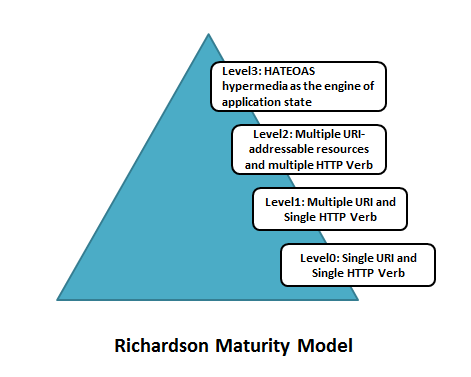
\includegraphics[width=\textwidth,height=\textheight,keepaspectratio]{figuras/richardson-maturity-model.png}
  }
  \caption{Modelo de Maturidade descrito por Richardson}
\end{figure}
